\documentclass{article}
\usepackage{listings}
\usepackage{color}
\usepackage{amsmath}
\usepackage{graphicx}
\usepackage{float}
\usepackage{amssymb}
\usepackage{mathtools,amssymb}
\usepackage{amsfonts}
\usepackage{amsthm}
\usepackage[linguistics]{forest}
\usepackage[utf8]{inputenc} 
\usepackage{chngcntr}

\usepackage[top=2in, bottom=1.5in, left=1in, right=1in]{geometry}
\usepackage{graphicx}
\usepackage{amsfonts}
\usepackage{amssymb}
\usepackage{amsmath}


\usetikzlibrary{quotes,arrows.meta}
\tikzset{
  annotated cuboid/.pic={
    \tikzset{%
      every edge quotes/.append style={midway, auto},
      /cuboid/.cd,
      #1
    }
    \draw [every edge/.append style={pic actions, densely dashed, opacity=0.5}, pic actions]
    (0,0,0) coordinate (o) -- ++(-\cubescale*\cubex,0,0) coordinate (a) -- ++(0,-\cubescale*\cubey,0) coordinate (b) edge coordinate [pos=1] (g) ++(0,0,-\cubescale*\cubez)  -- ++(\cubescale*\cubex,0,0) coordinate (c) -- cycle
    (o) -- ++(0,0,-\cubescale*\cubez) coordinate (d) -- ++(0,-\cubescale*\cubey,0) coordinate (e) edge (g) -- (c) -- cycle
    (o) -- (a) -- ++(0,0,-\cubescale*\cubez) coordinate (f) edge (g) -- (d) -- cycle;
    \path [every edge/.append style={pic actions, |-|}]
    (b) +(0,-5pt) coordinate (b1) edge ["\cubex \cubeunits"'] (b1 -| c)
    (b) +(-5pt,0) coordinate (b2) edge ["\cubey \cubeunits"] (b2 |- a)
    (c) +(3.5pt,-3.5pt) coordinate (c2) edge ["\cubez \cubeunits"'] ([xshift=3.5pt,yshift=-3.5pt]e)
    ;
  },
  /cuboid/.search also={/tikz},
  /cuboid/.cd,
  width/.store in=\cubex,
  height/.store in=\cubey,
  depth/.store in=\cubez,
  units/.store in=\cubeunits,
  scale/.store in=\cubescale,
  width=10,
  height=10,
  depth=10,
  units=cm,
  scale=.1,
}






\newcommand{\R}{\mathbb{R}}

\newcommand{\change}{\textcolor{blue}}
\newcommand{\argmin}{\mathop{\mathrm{arg\,min}}}
\newcommand{\argmax}{\mathop{\mathrm{arg\,max}}} 

\counterwithin*{section}{part}
\definecolor{mGreen}{rgb}{0,0.6,0}
\definecolor{mGray}{rgb}{0.5,0.5,0.5}
\definecolor{mPurple}{rgb}{0.58,0,0.82}
\definecolor{backgroundColour}{rgb}{0.95,0.95,0.92}
\lstdefinestyle{CStyle}{
    backgroundcolor=\color{backgroundColour},   
    commentstyle=\color{mGreen},
    keywordstyle=\color{magenta},
    numberstyle=\tiny\color{mGray},
    stringstyle=\color{mPurple},
    basicstyle=\footnotesize,
    breakatwhitespace=false,         
    breaklines=true,                 
    captionpos=b,                    
    keepspaces=true,                 
    numbers=left,                    
    numbersep=5pt,                  
    showspaces=false,                
    showstringspaces=false,
    showtabs=false,                  
    tabsize=2,
    language=C
}


\title{PLDAC - Etude de différentes techniques pour la classification de signaux d'EEG et MEG}
\author{Buton Nicolas}
\renewcommand{\contentsname}{Table des matières}
\begin{document}
\pagenumbering{gobble}
\maketitle
\begin{center}

\includegraphics[scale=1]{images/logoSorbonne.jpg}
\end{center}
\newpage
\tableofcontents
\newpage
\pagenumbering{arabic}
\part{Introduction}
Notre etude ce place dans le cadre de l'annalyse de série temporelle multivarier, qui comporte une dimension temporel et un spatiale.\\

Les interfaces cerveaux machines ont besoin de réagir vite et donc on doit analyser le signal sur un laps de temps court.\\

Historiquement cela ce faisait avec des méthodes linéaire, cela avait des performances assez faible et il fallait donc répéter l’expérience plusieurs fois comme c'est fait dans les méthodes P300(à détailler).

Barachant à ensuite proposer les méthodes riemannien qui sont plus robuste et qui ont permit d'attaquer des taches plus compliqué comme le transfert entre sujet.\\

Les signaux étudié seront des signaux d'Électroencéphalographie(EEG) et de Magnétoencéphalographie(MEG). Le premier consiste a enregistrer les signaux électrique a la surface du crane grâce a des électrodes, le second enregistre l'activité magnétique induite par l'activité des neurones grâce a un ensemble de magnétomètre.
\newline
\newline
L'une des difficultés pour traiter ces signaux est le fait que les électrodes ne sont jamais situées exactement au même endroit sur le crane entre chaque essai, et entre chaque personne. De plus il peut y avoir beaucoup de bruit généré par le matériel ou les mouvement de l'utilisateur par exemple.
\newline
\newline
Pour être résistant au bruit on a donc besoin de manipuler des matrices de covariance et pour cela un moyen est d'utiliser la géométrie de Riemann qui peut définir une distance entre matrice définit positive, les matrices de covariance font partie de ce groupe. La deuxième méthode consiste a aplatir la matrice.
\newline
\newline
C'est pour cela que dans les méthodes de l’état de l'art la géométrie riemannienne est utilisé. Ces méthode permette aussi un meilleur sucées pour le transfert d'un sujet à un autre.
\newline
\newline
Par la suite nous allons comparer ces méthodes avec de la géométrie riemannienne avec d'autres méthodes plus classique, ainsi qu'une méthode de deep learning.
\newline
\newline
Dans ce rapport nous étudierons nos méthodes sur 3 datasets différents : Eye close/eye open, brain invader et DecMeg2014.\\



\part{État de l'art - la géometrie de riemann}
\section{Distance}
Pour deux matrice $\mathbf{\Sigma}_1$ et $\mathbf{\Sigma}_2$ leurs distances est d’après la géométrie de Riemann est la suivante :\\
\begin{equation}
\label{eq:Rgeodistance}
\delta_R(\mathbf{\Sigma}_1,\mathbf{\Sigma}_2) 
= 
\Vert \mathrm{log} \left( \mathbf{\Sigma}_1^{-1/2} \mathbf{\Sigma}_2 \mathbf{\Sigma}_1^{-1/2} \right) \Vert_F
=
\left[ \sum_{c=1}^{C} \log^2 \lambda_c \right]^{1/2},
\end{equation}
où $\lambda_c, c=1\ldots C$ sont les valeurs propres réelles de $\mathbf{\Sigma}_1^{-1/2} \mathbf{\Sigma}_2 \mathbf{\Sigma}_1^{-1/2}$ et C le nombre d’électrodes.
\\
F :Norme de Frobenius

\section{Point moyen}
Pour définir la matrice moyenne nous ne possédons pas d'expression explicite.
\begin{equation}
\mathfrak{G} \left( \mathbf{\Sigma}_1,\ldots,\mathbf{\Sigma}_I \right) = \argmin_{\mathbf{\Sigma}} 
\sum_{i=1}^{I} 
\delta_R^2 \left( \mathbf{\Sigma},\mathbf{\Sigma}_i \right).
\label{eq:geo_mean}
\end{equation}
Pour la calculer on peut utiliser une descente de gradient.

\section{Espace tangent}
On peut projeter un point de l'espace de Riemann définit par une matrice NxN sur un espace tangent avec N(N+1)/2 dimensions.
\begin{figure}[H]
\begin{center}
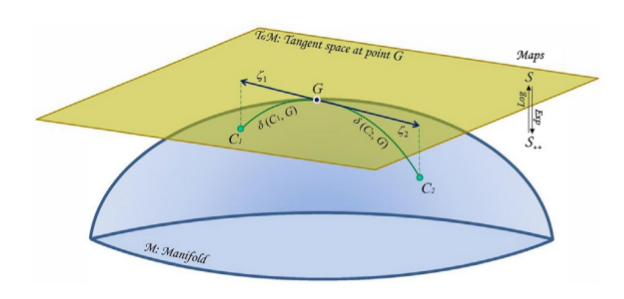
\includegraphics[scale=0.5]{images/Riemann_tangent_space.png}
\end{center}
\caption{Affichage del'espace tangent}
\end{figure}
Article sur la géométrie de Riemann : \\
- Brain invader \cite{congedo_brain_nodate} \\
- Geometrie de riemann \cite{congedo_riemannian_2017}\\


\part{Les différents modèles}
Nous allons représenter a l'aide d'un graphe les différentes méthodes que nous allons tester par la suite.
\begin{center}
\begin{forest}
[Brut
  [Filtre passe-bas
	[SVM(8)]  
	[KNN(9)]
  ]
  [TF
  	[SVM(1)]
  	[KNN(2)]
  ]
  [Cov
  	[SVM(3)]
  	[MDM(4)]
  	[KNN(5)]
  ]
  [SVM(6)]
  [KNN(7)]
  [CTR(8)]
]
\end{forest}
\end{center}

Légende :\\
Cov : Matrice de covariance\\
TF : Transformé de fourier\\
MDM : Minimum Distance to Mean\\
CTR : Chaine de traitement riemannienne, détaillé plus loin.
\\
Prédiction théorique : \\
La méthode 6 et 7 ne devrais pas fonctionner car avec une seule données c'est difficile de faire quoi que ce soit.\\
La méthode 8 et 9 ne devrais pas fonctionner car il n'y aura pas invariance par translation.\\
De plus nous introduirons une nouvelle méthode plus complexe dans le dernier dataset DecMeg2014.
\subsection{Format des données}
En entrée deux format sont possible. Le premier est une serie temporel pour chaque éléctrodes ainssi que les labels pour chaque données d'entrée.\\
Notons :\\
- C : le nombre de canaux.\\
- T : le temps écoulé en seconde pendant l'enregistrement des données.\\
- f : la fréquence d’échantillonnage du signal.\\
Nous dispossons donc d'une matrice de taille Cx(T*f), ainsi que d'un vecteur de label de taille (T*f).\\
Mais un deuxieme format d'entrée est possible, en découpant par trial, a chaque trial correspond un label.\\
Notons :\\
TT : le temps d'un trial.\\
NT : le nombre de trial.\\
Nous disposons donc d'un tenseur de taille (TT*f)xCxNT, et d'un vecteur de label de taille NT.\\
On peut passer du premier formalisme a l'autre en découpant par trial(en définissant une taille de fenêtre) mais nous avons plusieurs possibilité pour savoir quels labels associé a ce trial (label majoritaire,premier label,dernier label,etc...).\\
\subsection{Description des modèles}
\paragraph{1 et 2 - SVM et KNNavec une transformer de fourrier}
La première étape de notre modèle est d'effectuer une transformer de fourrier, c'est a dire passé d'un signal temporel à un signal fréquentiel. Pour calculer nous utiliserons l'algorithme FFT(Fast fourier transform).Nous garderons uniquement le modules pour rester avec des valeurs réelles plutôt que complexe.\\

Ensuite nous utilisons un SVM pour prédire les labels dans un cas et un KNN dans l'autre.
\paragraph{3,4 et 5 - SVM,MDM et KNN avec matrice de covariance }
Pour cette approche nous devons passer au deuxième format de données(décrit dans la partie précédente), si les données nous sont donné dans le premier format nous devons définir une taille de fenêtre et une méthode d'attribution des labels.\\
Ensuite on calcul la matrice de covariance :\\
$
\mathbf{\Sigma}_{i}=\frac{1}{C} \tilde{\mathbf{X}} \overline{\mathbf{X}}^{T}
$
Avec X ma matrice d'entrée.
\paragraph{6 et 7 - SVM et KNN sur les données brut}

\paragraph{8 et 9 - SVM et KNN avec un filtre passe bas}

\paragraph{8 - Chaine de traitement riemannienne}
1 - On garde uniquement 1 secondes sur les 1.5 secondes de signal car le stimulus intervient qu’après 0.5 secondes. \\
2 - On filtre le signal avec un filtre passe bande de Butterworth d'ordre 5 entre 1Hz et 20Hz.\\

\begin{figure}[H]
\begin{center}
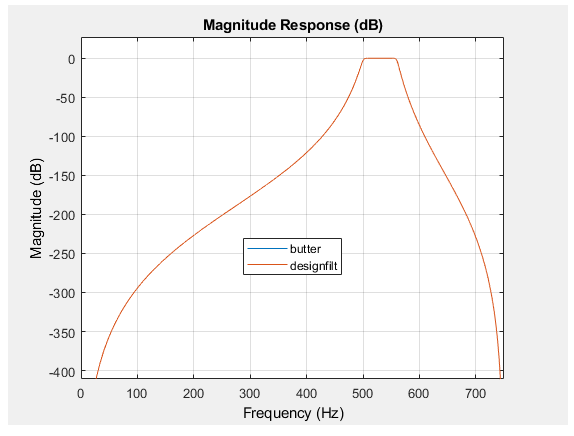
\includegraphics[scale=0.4]{images/butterworth_filter.png}
\end{center}
\caption{butterworth filter}
\end{figure}

3 - Par la suite on effectue un filtrage spatial, on extrait 4 channel virtuel par classe.\\
\begin{figure}[H]
\begin{center}
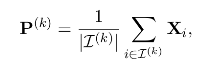
\includegraphics[scale=0.8]{images/P_moyen.png}
\end{center}
\caption{P moyen}
\end{figure}


\begin{figure}[H]
\begin{center}
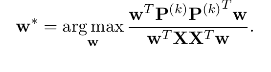
\includegraphics[scale=0.8]{images/spatial_filtering.png}
\end{center}
\caption{spatial filtering}
\end{figure}


\begin{figure}[H]
\begin{center}
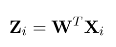
\includegraphics[scale=0.8]{images/Zi.png}
\end{center}
\caption{Zi}
\end{figure}


\begin{figure}[H]
\begin{center}
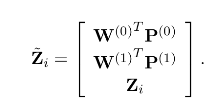
\includegraphics[scale=0.8]{images/features_space.png}
\end{center}
\caption{features space}
\end{figure}

\begin{figure}[H]
\begin{center}
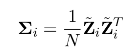
\includegraphics[scale=0.8]{images/covariance.png}
\end{center}
\caption{covariance}
\end{figure}


4 - On définit une nouvelle entrée comme étant la concaténation :\\
- du signal moyen de la classe 1 auquel on multiple par W0 pour les projeter sur les channels virtuelles appris précédemment.\\
- idem pour la classe 2\\
- Et ensuite le signal Xi projeter sur les 8 channels.\\
5 - On calcul la covariance de cette matrice.\\
6 - On projette cette matrice sur l'espace tangent.\\
7 - On estime pour les 15 autre sujets avec ce filtre spatial
8 - On fait la même chose pour les 15 autres sujet et on concaténe.\\
9 - Régression logistique avec une régularisation lasso.\\
Les figures suivantes représentes la forme des matrices au fur et a mesure du processus. Elles sont a lire de gauche a droite et de haut en bas.
\\
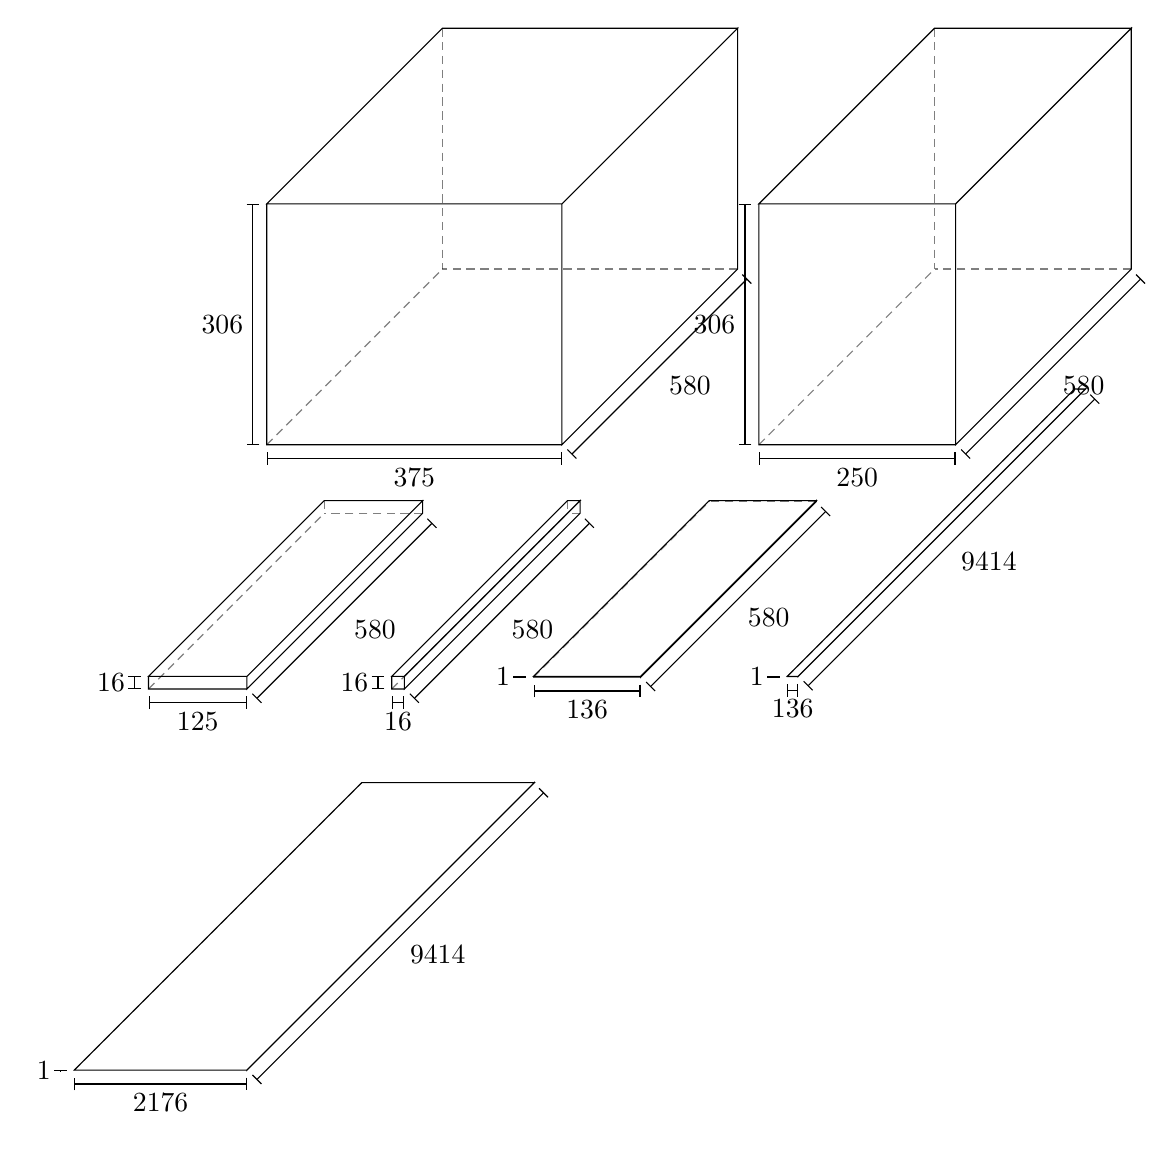
\begin{tikzpicture}
  \pic at (0,10) {annotated cuboid={width=375, height=306, depth=580, scale=.01, units=}};
  \pic at (5,10) {annotated cuboid={width=250, height=306, depth=580, scale=.01, units=}};
   \pic at (-4,4) {annotated cuboid={width=125, height=16, depth=580, scale=.01, units=}};
   \pic at (-2,4) {annotated cuboid={width=16, height=16, depth=580, scale=.01, units=}};
   \pic at (1,4) {annotated cuboid={width=136, height=1, depth=580, scale=.01, units=}};
   \pic at (3,4) {annotated cuboid={width=136, height=1, depth=9414, scale=.001, units=}};
   \pic at (-4,-1) {annotated cuboid={width=2176, height=1, depth=9414, scale=.001, units=}};
\end{tikzpicture}


\part{Experimentations}
\section{Prise en main sur un dataset simple}
\subsection{Decription du dataset eye close/eye open}
Ce dataset contient les données enregistré avec un casque EEG ou l'on a demandé au sujet d'ouvrir ou de fermer les yeux a certain moment. La tache a accomplir est de classifier a chaque enregistrement si la personne a les yeux ouvert ou fermé.\\
\\
Le signal est échantillonné à 512Hz. Il y a 7 femmes et 13 hommes pour un total de 20 participant pour ce dataset. L'age moyen est de 25.8 ans avec un écart type de 5.27 et une médiane a 25.5 ans. 18 sujets ont entre 19 et 28 ans et deux participants ont respectivement 33 ans et 44 ans.Le casque d'enregistrement est composé de 16 électrodes.\\
\\
On commence par visualiser le signal des 16 électrodes ainsi que leurs labels associé au cours du temps.\\
\begin{figure}[H]
\begin{center}
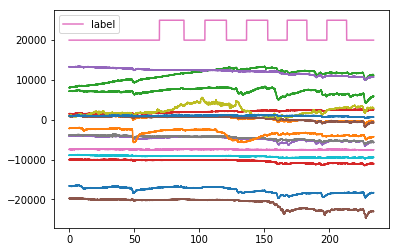
\includegraphics[scale=0.8]{images/donnees_entree.png}
\end{center}
\caption{Affichage des données brut}
\end{figure}

\subsection{Résultat des différents algorithmes}
\subsubsection{Valeurs de k pour les différents KNN}

\paragraph{KNN sur les données brut}
\begin{figure}[H]
\begin{center}
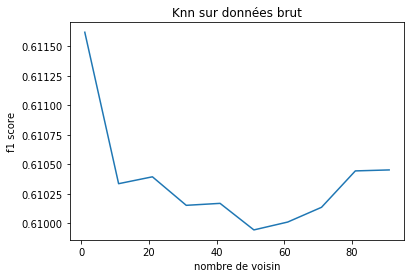
\includegraphics[scale=0.7]{images/f1_score_knn_brut.png}
\end{center}
\caption{F1 Score(en cross validation) du knn en fonction du pourcentage des données utilisé pour le train}
\end{figure}
$
neigh = KNeighborsClassifier(n_neighbors=10)
$


\paragraph{Riemann Cov KNN }
\begin{figure}[H]
\begin{center}
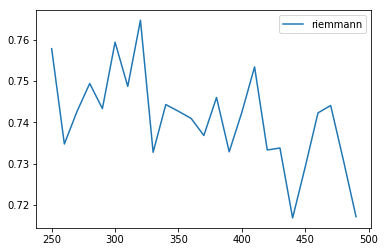
\includegraphics[scale=0.7]{images/riemann_cov_knn_f1Score.png}
\end{center}
\caption{F1 Score(en cross validation) du Riemann knn en fonction du nombre de données par paquet}
\end{figure}

estimer la matrice de covariance\\
$
cov = pyriemann.estimation.Covariances().fit_transform(X)
$
\\
validation croisée\\
$
knn = pyriemann.classification.KNearestNeighbor(n_neighbors=10)
$

\paragraph{KNN filtre passe bas }
\begin{figure}[H]
\begin{center}
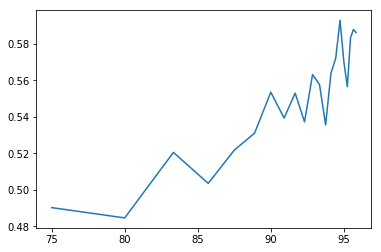
\includegraphics[scale=0.7]{images/knn_passe_bas_f1Score.png}
\end{center}
\caption{F1 Score(en cross validation) du knn en fonction du pourcentage des données utilisé pour le train}
\end{figure}

estimer la matrice de covariance\\
$
neigh = KNeighborsClassifier(n_neighbors=10)
    y_pred = cross_val_predict(neigh,donnees,labels,cv=k)
$
\\

\paragraph{KNN transformée de fourier }
\begin{figure}[H]
\begin{center}
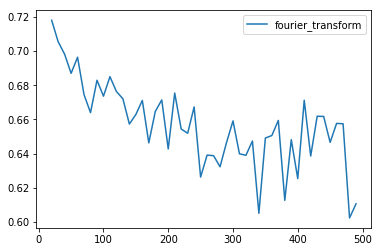
\includegraphics[scale=0.7]{images/knn_tf_f1Score.png}
\end{center}
\caption{F1 Score(en cross validation) du knn en fonction}
\end{figure}

estimer la matrice de covariance\\
$
cov = pyriemann.estimation.Covariances().fit_transform(X)
$
\\
validation croisée\\
$
knn = pyriemann.classification.KNearestNeighbor(n_neighbors=10)
$


\subsubsection{Etudes sur la longueur de la fennettre optimale}

\paragraph{SVM sur les données brut}
$
clf = SVM(max_iter=10000,shuffle=True)
$
Cross validation avec 5 parties :\\
F1 Score : 0.5390625

\paragraph{Riemann Cov MDM }
\begin{figure}[H]
\begin{center}
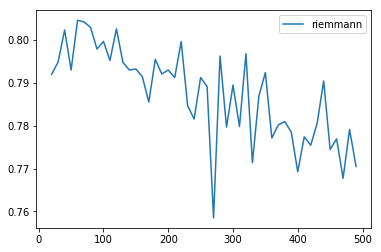
\includegraphics[scale=0.7]{images/riemann_cov_MDM_f1Score.png}
\end{center}
\caption{F1 Score(en cross validation) de riemann MDM en fonction du nombre de données par paquet}
\end{figure}

estimer la matrice de covariance\\
$
cov = pyriemann.estimation.Covariances().fit_transform(X)
$
\\
validation croisée\\
$
mdm = pyriemann.classification.MDM()
$


\paragraph{SVM filtre passe bas }
\begin{figure}[H]
\begin{center}
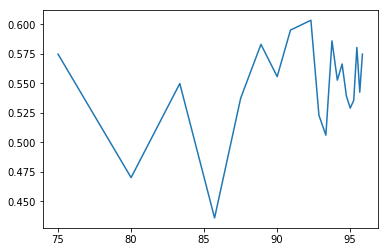
\includegraphics[scale=0.7]{images/perceptron_passe_bas_f1Score.png}
\end{center}
\caption{F1 Score(en cross validation) du SVM en fonction du pourcentage des données utilisé pour le train}
\end{figure}
modele :\\
$
 clf = SVM(max_iter=10000,shuffle=True)    
$


\paragraph{SVM transformée de fourier }
\begin{figure}[H]
\begin{center}
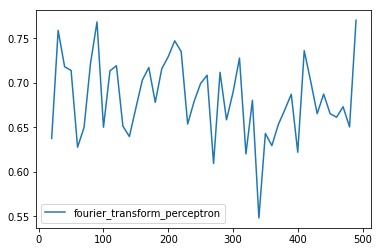
\includegraphics[scale=0.7]{images/perceptron_tf_f1Score.png}
\end{center}
\caption{F1 Score(en cross validation) du SVM en fonction de la taille de la fenêtre}
\end{figure}

estimer la matrice de covariance\\
$
cov = pyriemann.estimation.Covariances().fit_transform(X)
$
\\
validation croisée\\
$
knn = pyriemann.classification.KNearestNeighbor(n_neighbors=10)
$

\subsubsection{Tableau récapiltulatif}
f1-score arrondie à deux chiffre apres la virgule.\\
\begin{tabular}{|l|c|}
  \hline
  Nom de l'algorithme & f1-score\\
  \hline
  les données brut & 0.54 \\
  KNN sur les données brut & 0.61\\
  Riemann Cov MDM  & 0.84 \\
  Riemann Cov KNN & 0.77\\
  SVM filtre passe bas & 0.60 \\
  KNN filtre passe bas & 0.59 \\
  SVM transformée de fourier & 0.77 \\
  KNN transformée de fourier & 0.72 \\
  \hline
\end{tabular}

\section{Brain Invader}
\subsection{Description de la tache de machine learning}
Ce dataset à été enregistrer avec les sujets placer devant un pc ou une grille d'alien était représenté sur un écran.12 flashs dont 2 comprennent l'alien ciblé. Détecté les flash ou il y a l'alien en regardant l'activité cérébrale.Plusieurs tentative pour détruire l'alien.\\
Première tache : Classification binaire (le flash nous intéresse(il y a l'alien cible dedans) ou pas)\\
Deuxième tache : dans le groupe de 12 ou sont les deux flashs avec l'alien cible.\\


\begin{figure}[H]
\begin{center}
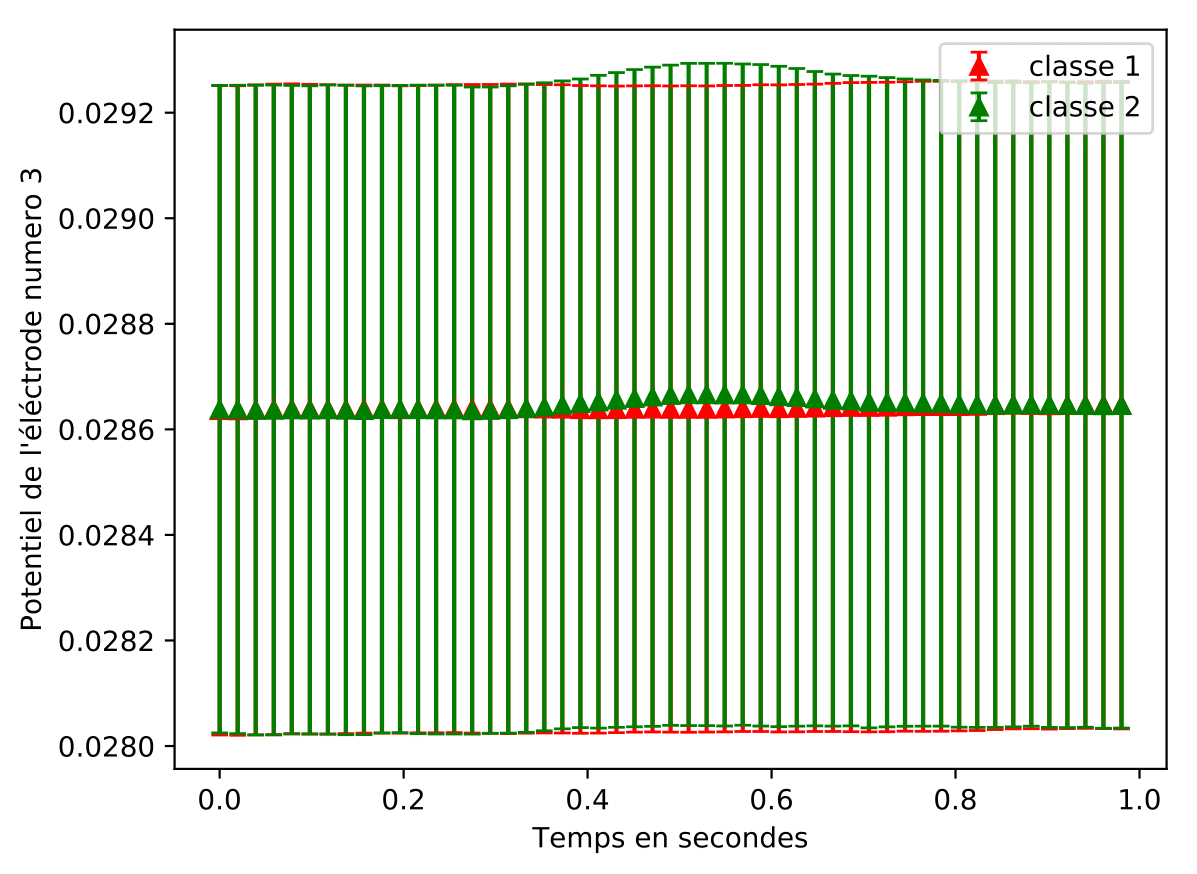
\includegraphics[scale=0.2]{images/visuel_classe_mean_std-1.png}
\end{center}
\caption{visuel classe mean std}
\end{figure}

\begin{figure}[H]
\begin{center}
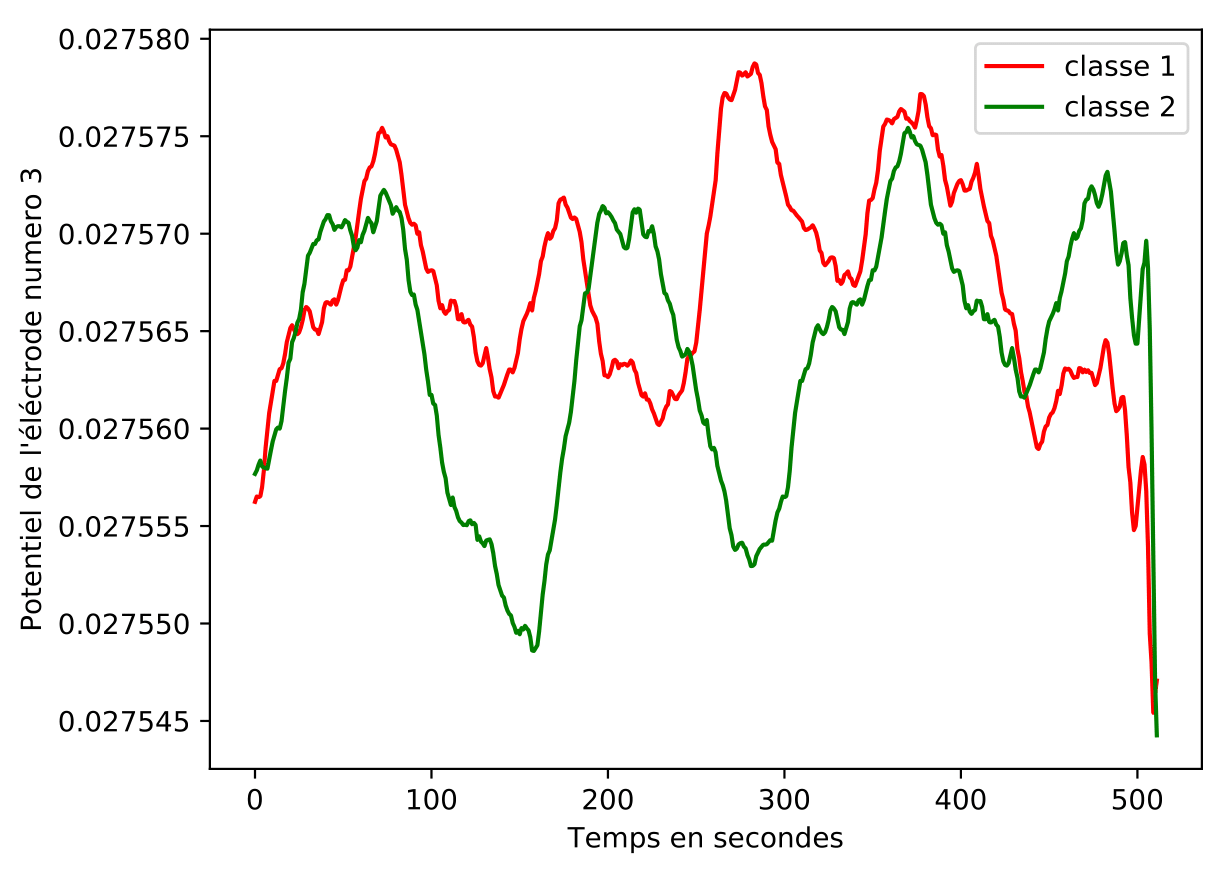
\includegraphics[scale=0.2]{images/visuel_data_0-1.png}
\end{center}
\caption{visuel data 0-1}
\end{figure}

F1-score des différents algorithme sur brain invader : \\
\begin{tabular}{|l|l|l|l|}
\hline
nom de l'algorithme                                                              & 1 seconde         & 0.1 seconde       & 0.04 seconde      \\
\hline
SVM brut      & 0.323051948051948 & 0.326461038961039 & 0.267532467532467 \\
SVM tf       & 0.451136363636364 & 0.323051948051948 & 0.408313347178491 \\
riemann MDM         & 0.441884775795033 & 0.450794330760887 & 0.441463342031226 \\
knn brut           & 0.391033345601445 & 0.421304978708651 & 0.477791812169029 \\
cov SVM       & 0.293170459768325 & 0.32987012987013  & 0.267283968878502 \\
passe bas KNN       & 0.468170847379269 & 0.417829605960706 & 0.467431891494059 \\
knn tf            & 0.399253802094698 & 0.470427433051929 & 0.453723364485908 \\
passe bas SVM & 0.267532467532467 & 0.326461038961039 & 0.451136363636364 \\
conv1D                & 0.384761943288956 & 0.326461038961039 & 0.33686397710642 \\
\hline
\end{tabular}
\\
Il n'a pas été possible de comparer les résultats avec les résultats de l'auteur du dataset car il manquait la composition des groupe d'alien qui clignotait.\\
\section{DecMeg2014}
\subsection{Description du dataset}
La tache que l'on doit réaliser avec le dataset DecMeg2014 est une classification binaire. Le but est de déterminer si le stimulus visuel est un visage clair ou un brouiller qui est montré au participant.L'activité de leurs cerveaux est enregistrer grâce à un appareil de magnetoencéphalographie. Cet appareil dispose de 306 magnétomètres.
\\
Ce dataset est extrait d'une compétition kaggle du même nom.
\\
23 sujets on participé à ce test avec environ 580 trials par sujet. Nous disposons de 16 sujets avec leurs labels associé et 7 sujets ou nous avons uniquement les données.
\subsection{Méthode d'évaluation}
Sur le dernier dataset DecMeg2014 nous disposons des données pour 16 sujets, nous procéderons donc comme décris ci-dessous pour l'évaluation de nos différentes méthodes :\\
- entrainement sur une partie de 1 et eval sur 1 (validation croisée sur un seul)\\
- entrainement sur 1 et évaluation sur tous les autres (16 expériences a faire)\\
- entrainement sur 15 et évaluation sur 1 (16 expériences a faire )\\
- entrainement sur 16 et eval sur 16 tout mélanger avec validation croisée.
\\
Ces façon d'évaluer nous permette de tester plusieurs caractéristique de nos modèles dont la capacité de transfert d'un sujet a l'autre.
\\
Pour chaque test on sauvegardera le f1 score sur la classe minoritaire.

\part{Conclusion}
D'après nos résultat nous pouvons conclure que....
\\
Il pourrais etre interessant de combiner des methodes de deep learning et de géometrie de riemann.
\bibliographystyle{ieeetr}
\bibliography{MyLibrary} 


\end{document}
